\documentclass[11pt, a4paper]{ctexart}

\usepackage{experiment_style}

\begin{document}

% =========================================
% P205. Q2
% =========================================
\begin{problem}{P205. Q2}
    炼钢厂出钢时所用的盛钢水钢包，在使用过程中由于钢液及炉渣对包衬耐火材料的侵蚀，使其容积不断增大。经试验，钢包的容积 $y$ 与相应的使用次数 $x$ 的数据如下：
    \[
        \resizebox{\textwidth}{!}{$
        \begin{array}{c|cccccccccccccc}
            x & 2 & 3 & 5 & 6 & 7 & 9 & 10 & 11 & 12 & 14 & 16 & 17 & 19 & 20 \\ \hline
            y & 106.42 & 108.26 & 109.58 & 109.50 & 109.86 & 110.00 & 109.93 & 110.59 & 110.60 & 110.72 & 110.90 & 110.76 & 111.10 & 111.30
        \end{array}
        $}
    \]
    试用最小二乘法求一形如
    \[
        y=\frac{x}{ax+b}
    \]
    的经验公式，并作出拟合图形。
\end{problem}

\begin{solution}
    \textbf{实验内容、步骤及结果}

    最小二乘矩阵函数 \texttt{chap-6/leastSquaresMatrix.m}：

\begin{lstlisting}[language=Matlab]
function [A, b] = leastSquaresMatrix(x, y, m)

    assert(length(x) == length(y), 'The lengths of x and y must be the same.');

    n = length(x);

    A = zeros(m + 1, m + 1);
    b = zeros(m + 1, 1);

    for i = 1:m + 1
        for j = 1:m + 1
            for k = 1:n
                A(i, j) = A(i, j) + x(k) ^ (i - 1 + j - 1);
            end
        end

        for k = 1:n
            b(i) = b(i) + y(k) * x(k) ^ (i - 1);
        end
    end
end
\end{lstlisting}

    主程序 \texttt{chap-6/P205\_Q2.m}：

\begin{lstlisting}[language=Matlab]
x = [2; 3; 5; 6; 7; 9; 10; 11; 12; 14; 16; 17; 19; 20];
y = [106.42; 108.26; 109.58; 109.50; 109.86; 110.00; 109.93; 110.59; 110.60; 110.72; 110.90; 110.76; 111.10; 111.30];
m = 1;

[A, b] = leastSquaresMatrix(1 ./ x, 1 ./ y, m);

coefficients = A \ b;

disp('y = x / ax + b');
disp('1/y = a + b/x');

disp('Coefficients:');
disp(coefficients);

a = coefficients(1);
b = coefficients(2);

figure;
scatter(x, y, 'filled');
hold on;

x_fit = linspace(min(x), max(x), 100);
y_fit = x_fit ./ (a * x_fit + b);
plot(x_fit, y_fit, 'r');

xlabel('x');
ylabel('y');
title('Data points and fitted line');
legend('Data points', 'Fitted line');
hold off;
\end{lstlisting}

    输出结果如下：

\begin{lstlisting}
>> P205_Q2
y = x / ax + b
1/y = a + b/x
Coefficients:
    0.0090
    0.0008
\end{lstlisting}

    拟合图像如下：

    \begin{figure}[htbp]
        \centering
        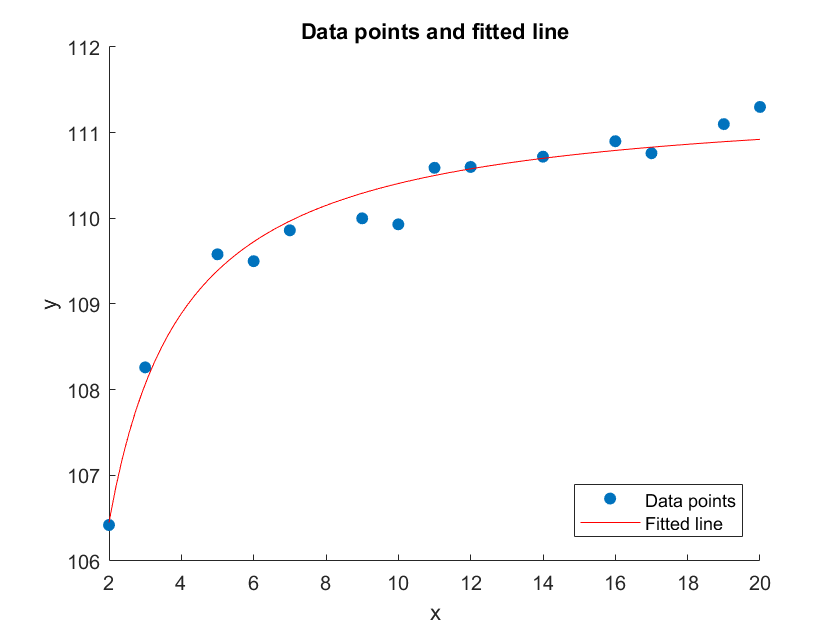
\includegraphics[width=0.80\textwidth]{../../bit-numerical-analysis-hw/chap-6/assets/P205_Q2.png}
    \end{figure}

    \textbf{实验结果分析}

    取变换
    \[
        \frac{1}{y}=a+\frac{b}{x},
    \]
    即对变量 $\left(\dfrac{1}{x},\dfrac{1}{y}\right)$ 作一次最小二乘拟合。实验结果给出
    \[
        a\approx 0.0090,\qquad b\approx 0.0008.
    \]
    因而经验公式可写为
    \[
        y\approx \frac{x}{0.0090x+0.0008}.
    \]
    从图像看，拟合曲线能够较好贴近数据点，说明该经验模型适合描述钢包容积随使用次数增加而逐渐趋于稳定的变化趋势。
\end{solution}


% =========================================
% 补充代码
% =========================================
\begin{problem}{补充代码}
    下面整理第 6 章相关题目的补充程序及运行结果。
\end{problem}

\begin{solution}
    \textbf{\texttt{chap-6/leastSquaresMatrix\_Func.m}}

\begin{lstlisting}[language=Matlab]
function [A, b] = leastSquaresMatrix_Func(H, g, int_a, int_b)
    % Number of basis functions
    n = length(H);

    % Initialize A and b
    A = zeros(n, n);
    b = zeros(n, 1);

    % Compute matrix A
    for i = 1:n
        for j = 1:n
            A(i, j) = integral(@(x) H{i}(x) .* H{j}(x), int_a, int_b, 'ArrayValued', true);
        end
    end

    % Compute vector b
    for i = 1:n
        b(i) = integral(@(x) H{i}(x) .* g(x), int_a, int_b, 'ArrayValued', true);
    end
end
\end{lstlisting}

    \textbf{P203\_Q1}

\begin{lstlisting}[language=Matlab]
x = [1.36; 1.49; 1.73; 1.81; 1.95; 2.16; 2.28; 2.48];
y = [14.094; 15.069; 16.844; 17.378; 18.435; 19.949; 20.963; 22.495];
m = 1;

[A, b] = leastSquaresMatrix(x, y, m);
coefficients = A \ b;

disp('x:');
disp(x);
disp('y:');
disp(y);
disp('m:');
disp(m);
disp('A:');
disp(A);
disp('b:');
disp(b);
disp('Coefficients:');
disp(coefficients);
\end{lstlisting}

\begin{lstlisting}
>> P203_Q1
A:
    8.0000   15.2600
   15.2600   30.1556

b:
  145.2270
  284.8363

Coefficients:
    3.9161
    7.4639
\end{lstlisting}

    \textbf{P203\_Q2}

\begin{lstlisting}[language=Matlab]
x = [1; 3; 4; 5; 6; 7; 8; 9; 10];
y = [10; 5; 4; 2; 1; 1; 2; 3; 4];
m = 2;

[A, b] = leastSquaresMatrix(x, y, m);
coefficients = A \ b;

disp('x:');
disp(x);
disp('y:');
disp(y);
disp('m:');
disp(m);
disp('A:');
disp(A);
disp('b:');
disp(b);
disp('Coefficients:');
disp(coefficients);
\end{lstlisting}

\begin{lstlisting}
>> P203_Q2
A:
           9          53         381
          53         381        3017
         381        3017       25317

b:
          32
         147
        1025

Coefficients:
   13.4597
   -3.6053
    0.2676
\end{lstlisting}

    \textbf{P203\_Q4}

\begin{lstlisting}[language=Matlab]
x = [19; 25; 31; 38; 44];
y = [19.0; 32.3; 49.0; 73.3; 97.8];
m = 1;

[A, b] = leastSquaresMatrix(x .^ 2, y, m);
coefficients = A \ b;

disp('y = a + bx^2');
disp('x:');
disp(x);
disp('y:');
disp(y);
disp('m:');
disp(m);
disp('A:');
disp(A);
disp('b:');
disp(b);
disp('Coefficients:');
disp(coefficients);
\end{lstlisting}

\begin{lstlisting}
>> P203_Q4
y = a + bx^2
A:
           5        5327
        5327     7277699

b:
   1.0e+05 *

    0.0027
    3.6932

Coefficients:
    0.9726
    0.0500
\end{lstlisting}

    \textbf{P203\_Q6}

\begin{lstlisting}[language=Matlab]
x = [1; 2; 3; 4; 5; 6; 7; 8];
y = [15.3; 20.5; 27.4; 36.6; 49.1; 65.6; 87.87; 117.6];
m = 1;

[A, b] = leastSquaresMatrix(x, log(y), m);
coefficients = A \ b;

disp('y = a*exp(bx)');
disp('ln(y) = ln(a) + bx');
disp('x:');
disp(x);
disp('y:');
disp(y);
disp('log(y)');
disp(log(y));
disp('m:');
disp(m);
disp('A:');
disp(A);
disp('b:');
disp(b);
disp('Coefficients:');
disp(coefficients);

a = exp(coefficients(1));
b = coefficients(2);

disp('a:');
disp(a);
disp('b:');
disp(b);
\end{lstlisting}

\begin{lstlisting}
>> P203_Q6
y = a*exp(bx)
ln(y) = ln(a) + bx
A:
     8    36
    36   204

b:
   29.9795
  147.1406

Coefficients:
    2.4367
    0.2913

a:
   11.4358

b:
    0.2913
\end{lstlisting}

    \textbf{P203\_Q7}

\begin{lstlisting}[language=Matlab]
x = [1; 2; 3; 4; 6; 8; 10; 12; 14; 16];
y = [4.00; 6.41; 8.01; 8.79; 9.53; 9.86; 10.33; 10.42; 10.53; 10.61];
m = 1;

[A, b] = leastSquaresMatrix(1 ./ x, 1 ./ y, m);
coefficients = A \ b;

disp('y = x / ax + b');
disp('1/y = a + b/x');
disp('x:');
disp(x);
disp('y:');
disp(y);
disp('1/x');
disp(1 ./ x);
disp('1/y');
disp(1 ./ y);
disp('m:');
disp(m);
disp('A:');
disp(A);
disp('b:');
disp(b);
disp('Coefficients:');
disp(coefficients);
\end{lstlisting}

\begin{lstlisting}
>> P203_Q7
y = x / ax + b
1/y = a + b/x
A:
   10.0000    2.6923
    2.6923    1.4930

b:
    1.2330
    0.4586

Coefficients:
    0.0789
    0.1649
\end{lstlisting}

    \textbf{P203\_Q12}

\begin{lstlisting}[language=Matlab]
% Define basis functions
H = {@(x) 1, @(x) x .^ 2, @(x) x .^ 4};

% Define target function
g = @(x) cos(x);

% Define integration interval
int_a = -pi / 2;
int_b = pi / 2;

[A, b] = leastSquaresMatrix_Func(H, g, int_a, int_b);
coefficients = A \ b;

disp('A:');
disp(A);
disp('b:');
disp(b);
disp('Coefficients:');
disp(coefficients);
\end{lstlisting}

\begin{lstlisting}
>> P203_Q12
A:
    3.1416    2.5839    3.8252
    2.5839    3.8252    6.7417
    3.8252    6.7417   12.9380

b:
    2.0000
    0.9348
    0.9585

Coefficients:
    0.9996
   -0.4964
    0.0372
\end{lstlisting}
\end{solution}

\end{document}
